\documentclass{report}
\usepackage{graphicx} % Required for inserting images
\usepackage{tabularx}
\usepackage[spanish]{babel}
\usepackage{minitoc}
\usepackage{etoc}
\usepackage{tikz}
\usepackage{amsmath}
\usepackage[style=ieee]{biblatex}

\addbibresource{intros.bib}
\addbibresource{cap1.bib}
\addbibresource{desordenados.bib}

\usepackage{hyperref}
\usepackage{csquotes}

\usepackage{hanging}

% Configuración para que todos os parágrafos teñan sangría francesa




\title{Apuntes segunda parte PDL}
\author{Marcelo F.M.}
\date{\today}

\def\profundidadIndice{section}
\def\profundidadIndiceCapitulo{subsubsection}

\begin{document}



\maketitle

\dominitoc

\etocsetnexttocdepth{\profundidadIndice}
\etoctableofcontents

\clearpage

\section{Definiciones}
Se entienden por usadas las siguientes definiciones:

\paragraph{Actos del habla:} Acciones que se llevan a cabo al pronunciar una frase, como «Prometo estar allí» o «Por favor, estate allí». Transmiten fuerzas ilocucionarias como prometer o pedir, que sitúan el contenido de la frase en un contexto de discurso con referencia a los estados mentales del hablante y del oyente y a los objetivos o acciones que la emisión de la frase consigue en el discurso. (traducido)\autocite{Daniel.AOS}

\paragraph{Ambiguo:} Que puede entenderse de varios modos o admitir distintas interpretaciones y dar, por consiguiente, motivo a dudas, incertidumbre o confusión. \autocite{rae.diccionario}

\paragraph{Anáfora:} Relación de identidad que se establece entre un elemento gramatical y una palabra o grupo de palabras nombrados antes en el discurso; p. ej.,  \textit{lo} y \textit{que había estado allí} en \textit{Dijo que había estado allí, pero no me lo creí.} \autocite{rae.diccionario}

\paragraph{Característica (Feature): } Cada palabra única del corpus se considera una característica.\autocite{diapos1}

\paragraph{Corpus:} Colección de todos los documentos presentes en nuestro conjunto de datos.\autocite{diapos1}

\paragraph{Dependencia:}
 Relación de origen o conexión / Relación de subordinación.\autocite{rae.diccionario}

\paragraph{Documento:}
 Conjunto de datos con la información a procesar.\autocite{diapos1}

\paragraph{Fonética:} Perteneciente o relativo a los sonidos del habla, conjunto de los sonidos de un idioma. \autocite{rae.diccionario}

\paragraph{Fonología:} Parte de la gramática que estudia cómo se estructuran los sonidos y los elementos suprasegmentales de una lengua para transmitir significados.\autocite{rae.diccionario}

\paragraph{Lenguaje natural:} Forma de lenguaje humano o una variedad lingüística generada espontáneamente en un grupo de hablantes con propósito de comunicarse.\autocite{wikipedia.es.lenguanatural}

\paragraph{Lexema:} Unidad mínima con significado léxico que no presenta morfemas gramaticales; p. ej., \textit{sol}, o que, poseyéndolos, prescinde de ellos por un proceso de segmentación; p. ej., \textit{terr}, en \textit{enterráis.} \autocite{rae.diccionario}

\paragraph{Morfema:} Unidad mínima aislable en el análisis morfológico. \autocite{rae.diccionario}

\paragraph{Morfología:}Parte de la gramática que estudia la estructura de las palabras y de sus elementos constitutivos. \autocite{rae.diccionario}

\paragraph{Ontología:} La ontología captura el conocimiento en ámbitos relacionados, proporciona una comprensión común del conocimiento de dominio, identifica vocabularios comunes de reconocimiento y ofrece una definición clara de la relación entre estos vocabularios desde distintos niveles de patrones formales. (traducido)\autocite{feng2007ontology}

\paragraph{Part of speech (POS):} Antigua clasificación de las palabras según su tipo. Modernamente el término «categoría gramatical» se refiere a una variable lingüística que puede tomar diferentes valores que condicionan la forma morfológica concreta de una palabra.\autocite{eswiki:159789898}  

\paragraph{Pragmatica:} Disciplina que estudia el lenguaje en su relación con los hablantes, así como los enunciados que estos profieren y las diversas circunstancias que concurren en la comunicación.\autocite{rae.diccionario}

\paragraph{Procesamiento del lenguaje natural o NLP:} Subcampo de la Inteligencia Artificial que se ocupa de las interacciones entre los ordenadores y los
lenguajes humanos (naturales).

\paragraph{Semántica:} Disciplina que estudia el significado de las unidades lingüísticas y de sus combinaciones.\autocite{rae.diccionario}

\paragraph{Sintaxis:} Parte de la gramática que estudia el modo en que se combinan las palabras y los grupos que estas forman para expresar significados, así como las relaciones que se establecen entre todas esas unidades. / Conjunto de reglas que definen las secuencias correctas de los elementos de un lenguaje de programación.\autocite{rae.diccionario}

\paragraph{Sistema determinista:} Sistema en el cual cada estado futuro del sistema está determinado por el previo. \autocite{wikipedia.es.sistemadeterminista}



\chapter{Un acercamiento}
\etocframedstyle[1]{}
\etocsetnexttocdepth{\profundidadIndiceCapitulo}
\localtableofcontents
\section{Introducción}
El procesamiento de lenguaje natural es un área de la
inteligencia artificial que estudia la comunicación entre las
personas y los ordenadores utilizando lenguas naturales.
Algunas de las aplicaciones típicas del PLN son:
\begin{itemize}
    \item Reconocimiento del habla
    \item Generación automática de resúmenes
    \item Traducción automática
    \item Detectar Spam u otros tipos de correspondencia no deseada
    \item Reconocer entidades en textos
    \item Responder a preguntas
    \item Autocompletar y/o rellenar textos
    \item Corregir textos
    \item Voz a texto
    \item Análisis de sentimientos
\end{itemize}

El «proceso del PLN» contempla 9 tipos de análisis sobre la entrada de un texto:
\begin{enumerate}

    \item {Fonológico}
    \begin{enumerate}
        \item Aplicado sobre lenguaje oral.
        \item Procesado de sonidos y ruidos.
    \end{enumerate}

    \item {Textual + Morfológico} 
        \begin{enumerate}
            \item Identifica tokens y tipos de palabras.
            \item Realiza POS tagging (etiquetado gramatical).
            \item Resuelve ambigüedades según el contexto.
            \item Determina formas, clases o categorías gramaticales de cada palabra.
            \item Para hacer la clasificación morfológica, puede usar formarios, diccionarios de morfemas, reglas de combinación y/o variaciones fonológicas. 
        \end{enumerate}

    \item{Léxico}
    \begin{enumerate}
        \item Distingue entre subtipos de palabras.
        \item Detecta grupos por significado.
        \item Genera información útil para análisis posteriores.
    \end{enumerate}
        
    \item {Sintáctico}
    \begin{enumerate}
        \item Establece relaciones de dependencia entre palabras.
        \item Analiza el orden y estructura de la oración.
        \item Desambigua palabras con múltiples funciones gramaticales.
        \item El significado depende de la estructura sintáctica.
    \end{enumerate}

    \item{Lógico}
    \begin{enumerate}
        \item Extrae significado de las oraciones usando lenguajes formales.
        
    \end{enumerate}
    
    \item {Semántico}
    \begin{enumerate}
        \item Desambigua palabras con múltiples significados.
        \item Utiliza información contextual.
        \item Implementa métodos basados en frecuencias y/o conocimiento del dominio.
    \end{enumerate}
    
    \item {Pragmático}
    \begin{enumerate}
        \item Más complejidad con semántico.
        \item Interpreta significado según el contexto.
        \item Va más allá de la estructura literal.
        \item Considera el entorno donde se emiten las oraciones.
    \end{enumerate}

    \item{Ilocutivo:} Analiza las intenciones.
    
\end{enumerate}

\section{Tipos de procesado del leguaje natural: Basado en reglas vs Estadístico}
Como el lenguaje natural es no-determinista \footnote{Un modelo determinista producirá siempre la misma salida a partir de las mismas condiciones de partida o el estado inicial}, no se puede procesar cual lenguaje formal. Por eso, hay que buscar técnicas para procesarlo.

Para ello, hay dos acercamientos principales: el uso de reglas y la predicción estadística.

\subsection{Basado en reglas}
Con una forma de procesar similar a las gramáticas usadas para lenguajes formales, este enfoque usa normas predefinidas para determinar los resultados.

Este usa una «suerte» de «sentido común». Requiere un esfuerzo manual para escribir las reglas y puede llevar algo más de tiempo.

\subsubsection{Ventajas}
\begin{itemize}
    \item Flexible.
    \item Fácil depuración.
    \item No requiere un entrenamiento intensivo.
    \item Tiene alta precisión.
\end{itemize}

\subsubsection{Desventajas}
\begin{itemize}
    \item Requiere de conocimientos técnicos.
    \item No permite cubrir todo el lenguaje.
\end{itemize}

\subsection{Predicción basado en estadística}
Extrae «conclusiones» a partir de los datos.
Este usa algoritmos de aprendizaje automático.
Una vez entrenado, este produce con positividad «deducciones» a partir de los datos.

\subsubsection{Ventajas}
\begin{itemize}
    \item Fácil escalabilidad.
    \item Aprendizaje automático.
    \item Desarrollo fácil y accesible.
    \item Puede proveer una cobertura extensa y hasta incluso completa del lenguaje.
\end{itemize}

\subsubsection{Desventajas}
\begin{itemize}
    \item Puede tener problemas para tener en cuenta el contexto.
    \item Necesita un volumen elevado de datos.
    \item Muy difícil de depurar.
\end{itemize}

\section{Ambigüedades}
Antes de empezar a trabajar con el texto, hay que procesarlo.
Sin embargo, hay una característica que puede dificultar la compresiónn de un texto: la ambigüedad.

Existen 5 tipos de ambigüedades:
\begin{enumerate}
    \item {Léxica:}        Ej: polisemia
    \item {Sintáctica:}    Una \textbf{frase} tiene múltiples interpretaciones. 
    \item {Semántica:}     \textbf{Parte de la oración} puede ser confundida o mal asociada.
    \item {Anafórica:}     Anáforas \textbf{dependientes del contexto} son usadas.
    \item {Pragmática:}     El significado \textbf{completo} de la frase depende del contexto que la contiene.
\end{enumerate}

Esto implica que, para evitar las ambigüedades, 
tendremos que tener ciertos conocimientos a la hora de emprender el procesado de la información.
Estos se podrían resumir como:

\begin{enumerate}
    \item La fonética y fonología de las palabras
    \item{Morfológico:} Como se \textquote{construyen} las palabras.
    \item{Sintáctico:} Como están estructuradas las oraciones y discursos.
    \item{Semántico:} El significado de las distintas unidades lingüísticas (palabras y oraciones).
    \item{Pragmático:} Como utilizar las palabras y oraciones según contexto.
    \item{Discursivo:} Saber como encajan las frases vinculadas entre ellas, lo que implica comprender vínculos pasados entre oraciones previas en el mismo documento.
    \item{Léxico:} Comprender las palabras del vocabulario.
\end{enumerate}

\section{Normalización}

Para poder análizar los textos de forma más \textquote{fácil}, a veces se requiere de reestructuraciones. Normalización:

\subsection{Preprocesado y limpieza}
\begin{itemize}
    \item Pasar el texto a minúsculas.
    \item Eliminar Stopwords. 
    Esto reduce mucho dimensionalidad y ruido.
    \item Eliminar y/o procesar etiquetas y trazas de HTML.
    \item Quitar símbolos de acentuación.
    \item Eliminar caracteres especiales no deseados.
    \item Corregir la ortografía de un texto.
    \item Expandir y/o normalizar palabras \textquote{especiales} como acrónimos.
\end{itemize}

\subsection {Tokenización}

\begin{itemize}
    \item División del texto en componentes básicos
    \item Identifica palabras y signos de   puntuación
    \item Maneja casos especiales como abreviaturas
    \item Existen casos difíciles en  los separadores
\end{itemize}

\subsection{Segmentación}
\begin{itemize}
    \item Separa texto en unidades independientes
    \item Divide en párrafos u oraciones (normalmente)
\end{itemize}

\subsection{Stemming}
Consiste en \textquote{despojar} a una palabra de sus  prefijos y sufijos para obtener una raíz aproximada. Reduce la dimensión del texto al haber más coincidencias.
\subsection{Lematización}
Devuelve una palabra a su lema o forma canónica. 
Esta técnica reduce dimensionalidad y ruido.
Por ejemplo, de \textit{carrera}, obtendríamos \textit{carro}.

\subsection{Etiquetado Gramatical (POS Tagging)}
\begin{itemize}
    \item Asigna categorías gramaticales a cada token (sub,verb,adj,...)
    \item Resuelve ambigüedades contextuales
\end{itemize}

\section{Word Embeddings}
Una de las formas de representar las palabras son los \textquote{\textit{Word-Embeddings}}.  Estos son representaciones vectoriales densas de palabras en un espacio continuo, donde las palabras con significados similares están cerca entre sí.
Generalmente, esto se hace con vectores de números, cuya \textbf{dimensión} depende del tamaño del vocabulario.

Su uso mejora el procesado de la información y existen 2 tipos: \textbf{estadísticos} y \textbf{predictivos}.

Unas de las técnicas usadas para los modelos estadísticos son:

\subsection{Técnicas para representación vectorial}
% \etocsettitle{Tipos de técnica}
% \etocsetstyle {}
\etocsettocdepth{subsubsection}
\etocsettocstyle{\centering\subsubsection*{Técnicas}}{}
\localtableofcontents

\subsubsection{One Hot Encoding}
Consiste en codificar las palabras en un vector de números base dos (binario).
De esta forma, se le asocia un identificador unívoco a cada palabra.

Esta técnica tiene como puntos negativos que, por un lado, tendrá una gran complejidad espacial. Además, ignora el contexto.

\subsubsection{Count-Vectorizer}
Consiste en crear una matriz que cruza variables (generalmente documento/palabra) y que tiene como valores la frecuencia de la variable fila en la variable columna.
Un ejemplo sería el visible en la \autoref{tab:ejcv}, en la que se mira en un conjunto hipotético de documentos sobre la alimentación en España y Bélgica las palabras \textquote{\textit{queso}} y \textquote{\textit{tofu}}.

\begin{table}[ht]
    \centering
    \begin{tabular}{ccc}
         & España & Bélgica \\
        Queso & 0.68 & 0.6 \\
        Tofu  & 0.32 & 0.4 \\
    \end{tabular}
    \caption{Ejemplo de Count-Vectorizer}
    \label{tab:ejcv}
\end{table}

Las frecuencias se denominan \textquote{frecuencia de términos}.

\subsubsection{Bag Of Words (BOW)}
Convierte un corpus a un vector de palabras con características sin repeticiones ordenado alfabeticamente, que son evaluadas con valores numéricos (índices), que indican la posición de estas palabras.
El valor asociado a cada posición es el número de apariciones de la palabra correspondiente.
Requiere de que se \textbf{tokenice} y \textbf{vectorice} previamente.

Ejemplo:
Voy a comprar pan a la  panadería.

\begin{table}[ht]
    \centering
    \begin{tabular}{ |c|ccccc|}
    \hline
                    & a & comprar & la & panadería & voy \\
    \hline
        Documento 1 & 2 & 1       & 1  & 1         & 1 \\
    \hline
    \end{tabular}
    \caption{ejemplo de bag of words}
    \label{tab:bow}
\end{table}

Como desventajas, no conserva el orden original en el vector y, dificulta o incluso bloquea futuros procesados o trabajos de PLN.

\subsubsection{N-Gramas}
Genera una matriz con todos los términos, con recuento por celda.
Esto lo hace basándose en el número $N$, que determina cuantas unidades entran en cada término. 

Las unidades van \textquote{encadenadas}, es decir, que si tuviéramos la cadena \textit{A B C D}, y pusiéramos $N=2$, tendríamos $\{(A,B),(B,C),(C,D)\}$

Cuando $N=1$, se considera un caso especial y se denomina \textquote{Vectorización por recuento}.

Ventajas de esta técnica son que mantiene el orden original y puede tener buena eficiencia. Además, al evitar la morfología del lenguaje la hace muy robusta.

Para aprovecharse de esa segunda ventaja, hay que escoger una buena $N$.
Si esta es muy pequeña, faltará información. Mas si escogemos una muy grande, habrá una saturación de información, que será más cara de procesar y peor.

Por lo tanto, la desventaja en este caso, será la dificultad para encontrar una $N$ adecuada.

\subsubsection{TF-IDF}
En inglés \textit{Term frequency - Inverse document frequency}.
Es una versión extendida del modelo Bolsa de Palabras, permite disminuir el peso de las palabras muy comunes en la colección de documentos.
Se puede dividir en dos partes:
\paragraph{TF:} 
\textit{Term frequency} o frecuencia del término.

Sean:
\[t\quad\text{Término}\]
\[d\quad\text{documento}\]
\[n\quad\text{Número de apariciones en el documento}\]
Tenemos la fórmula:
\[tf(t,d)=\frac{n_t}{\Sigma_{k=0}^{N} n_k}\]
Para esta fórmula, todos los términos \textit{tienen la misma importancia}

\paragraph{IDF:}
\textit{Inverse document frequency} o frecuencia inversa de documento.
Evalúa cuan importante es un término en un documento.
Su valor solo cambia entre términos.
sea $D$ un documento y $|D|$ la cardinalidad de los documentos,
\[idf(t,D)=\log_{10}\frac{|D|}{| \{d_i \in D | t \in d_i\}|}\]
Para calcular el tf-idf de una palabra sobre el corpus:
\[tf\_idf(t,d)=tf(t,d)*idf(t)\]
A valor más alto, mayor importancia tendrá el término.

Las ventajas de tanto BoW como TF-IDF, son su facilidad de implementación y sus buenos resultadps en clasificación de textos.

Sus desventajas son la falta de información semántica, su gran dimensionalidad y que no tengan en cuenta la posición en el texto de las palabras.

\section{Topic Modelling (LDA)}
Latent Dirichlet Allocation (LDA) es un algoritmo utilizado en el modelado de temas, una técnica estadística que identifica automáticamente los temas dentro de un conjunto de documentos. Los principales puntos son:
\begin{enumerate}
\item{\textbf{Objetivo}:} Clasificar el contenido textual (documentos, párrafos o frases) en temas, asignando probabilidades a palabras para cada tema y a temas para cada documento.

\item{\textbf{Funcionamiento}:}
\begin{itemize}
    \item Se calcula la probabilidad de que un tema $t$ esté presente en un documento $d$ ($P(t|d)$).
    \item Se evalúa la probabilidad de que una palabra $w$ esté asociada a un tema $t$ ($P(w|t)$).
    \item Ambas probabilidades se combinan iterativamente para ajustar la clasificación de temas.
\end{itemize}

\item{\textbf{Proceso}:}
\begin{enumerate}
    \item Preparación del texto: Incluye tokenización, eliminación de signos de puntuación y palabras irrelevantes, y procesos de stemming o lematización.
    \item Clasificación inicial: Se distribuyen palabras y temas en los documentos de forma inicial.
    \item Iteración: Las probabilidades se refinan en múltiples ciclos para mejorar la precisión.
\end{enumerate}

\item{\textbf{Ventajas}:} LDA es útil para identificar patrones temáticos en grandes cantidades de texto de manera no supervisada.

\item{\textbf{Ejemplo intuitivo}:} Similar a etiquetar fotos en categorías como "campo" o "ciudad" según las características dominantes (como "árboles" o "edificios"), las palabras se asignan a temas con base en su relevancia estadística.
\end{enumerate}

\section{Librerías}
\subsection{Listado de las librerías}

\etocsettocdepth{subsubsection}
\etocsettocstyle{\centering\subsubsection*{Librerías}}{}
\etocinline\localtableofcontents

\subsubsection{NLTK}
Creada en 2001 con fines educativos

Funcionalidades:
\begin{itemize}
    \item Tokenización.
    \item Etiquetado de partes del lenguaje (POS).
    \item Reconocimiento de Entidades Nombradas (NER).
    \item Clasificación.
    \item Análisis de sentimiento.
    \item Paquetes de chatbots.
    \item Aplicaciones
    \item Sistemas de recomendación.
    \item Análisis de sentimiento.
    \item Construcción de chatbots
\end{itemize}.


Ventajas:
\begin{itemize}
    \item Más de 50 corpus integrados
    \item Instalación sencilla vía pip
    \item Documentación extensa y ejemplos paso a paso
    \item Integración con etiquetador Stanford
\end{itemize}

Limitaciones para español:

\begin{itemize}
    \item Requiere entrenamiento con corpus cess\_esp (500,000 palabras)
    \item No incluye lematización
    \item Muchas funciones solo disponibles para inglés
\end{itemize}

Usa etiquetas EAGLES para POS tagging.

\subsubsection{Freeling}
Desarrollado por TALP (Universidad Politécnica de Catalunya)

Ventajas:

\begin{itemize}
    \item Soporte nativo para español
    \item Análisis morfológico completo
    \item Recursos lingüísticos adaptables
    \item Arquitectura cliente-servidor en C++
\end{itemize}

Desventajas:

\begin{itemize}
    \item Instalación compleja en Windows
    \item Requiere API para Python
    \item Necesita servidor en ejecución
\end{itemize}

Usa etiquetas EAGLES y tiene lematización

\subsubsection{Pattern.es}
Funcionalidades:
\begin{itemize}
    \item Conjugación de verbos
    \item Singularización/pluralización
    \item División de chunks
    \item POS tagging
\end{itemize}

Ventajas:
\begin{itemize}
    \item Instalación simple
    \item API intuitiva
    \item No requiere configuración adicional
\end{itemize}

Usa Penn TreeBank tags.

\subsubsection{SpaCy}

Funcionalidades:
\begin{itemize}
    \item Tokenización.
    \item Etiquetado de partes del lenguaje (POS).
    \item Reconocimiento de entidades con nombre (NER).
    \item Clasificación.
    \item Análisis de sentimientos.
    \item Análisis de dependencia.
    \item Vectores de palabras.
\end{itemize}

Aplicaciones:

\begin{itemize}
    \item Autocompletar y autocorregir.
    \item Análisis de reseñas.
    \item Resumir.
\end{itemize}

Características principales:

\begin{itemize}
    \item Modelos estadísticos pre-entrenados
    \item Vectores de palabras
    \item Soporte para 45+ idiomas
    \item Integración con deep learning
    \item Funcionamiento basado en «tuberías»
\end{itemize}

Ventajas:

\begin{itemize}
    \item Instalación simple vía pip
    \item Alto rendimiento
    \item Etiquetado POS completo (tiempo, género, número, etc.)
    \item Basado en OntoNotes5
\end{itemize}

Usa Penn TreeBank para POS tagging

\subsubsection{Stanford NLP}
Framework Java con API para Python

Funcionalidades:

\begin{itemize}
    \item Tokenización
    \item Análisis morfológico
    \item Reconocimiento de entidades
    \item Análisis sintáctico con árboles de dependencia
\end{itemize}

Limitaciones:

\begin{itemize}
    \item Requiere Java Runtime
    \item Configuración de variables de entorno
    \item Servidor Java en segundo plano
\end{itemize}

Usa etiquetas EAGLES y tiene lematizador

\subsubsection{Gensim}
Funcionalidades:
\begin{itemize}
    \item Word embeddings 
    \item Análisis semántico latente.
    \item Factorización de matrices no negativas.
    \item TF-IDF.
\end{itemize}

Aplicaciones:

\begin{itemize}
    \item Conversión de documentos en vectores.
    \item Búsqueda de similitudes textuales.
    \item Resumen de textos.
\end{itemize}

\subsubsection{TextBlob}
TextBlob es una librería de Python diseñada principalmente para el procesamiento de datos textuales. 
Basada en NLTK.

Funcionalidades:

\begin{itemize}
    \item Etiquetado de parte del discurso.
    \item Extracción de frases sustantivas.
    \item Análisis de sentimiento.
    \item Clasificación.
    \item Traducción de idiomas.
    \item Análisis sintáctico.
    \item Integración de redes de palabras.
\end{itemize}

Aplicaciones:

\begin{itemize}
    \item Análisis de sentimientos.
    \item Corrección ortográfica.
    \item Traducción y detección de idiomas.
\end{itemize}

\subsubsection{Stanza}
Stanza es una herramienta integral diseñada para realizar análisis lingüísticos avanzados en múltiples idiomas. 
Desde procesar texto sin formato hasta llevar a cabo análisis sintácticos y extraer entidades nombradas, 
Stanza proporciona modelos de Procesamiento del Lenguaje Natural (PLN) modernos y eficientes.

\begin{itemize}
    \item \textbf{Principales características:}
    \begin{itemize}
        \item Utiliza redes neuronales completas para garantizar un análisis robusto, ofreciendo capacidades como:
        \begin{itemize}
            \item Segmentación del texto (tokenización),
            \item Manejo de tokens compuestos (expansión MWT),
            \item Obtención de la forma base de las palabras (lematización),
            \item Identificación de categorías gramaticales (POS) y análisis morfológico,
            \item Determinación de relaciones gramaticales (análisis de dependencias),
            \item Identificación de nombres propios y otros elementos clave (reconocimiento de entidades nombradas).
        \end{itemize}
        \item Ofrece modelos preentrenados que son compatibles con 66 idiomas, garantizando una cobertura lingüística extensa.
    \end{itemize}
\end{itemize}


Funcionalidades:

\begin{itemize}
    \item Etiquetado de parte del discurso.
    \item Extracción de frases sustantivas.
    \item Análisis de sentimiento.
    \item Clasificación.
    \item Traducción de idiomas.
    \item Análisis sintáctico.
    \item Integración de redes de palabras.
\end{itemize}

Aplicaciones:

\begin{itemize}
    \item Análisis de sentimientos.
    \item Corrección ortográfica.
    \item Traducción y detección de idiomas.
\end{itemize}

\subsection{Comparación}
Comparación de características clave:

\begin{tabularx}{\linewidth}{|X|X|X|X|X|X|} 
\hline
Herramienta & Código & Segmentación y \newline tokenización & Etiquetado POS & Lematización \\ 
\hline 
NLTK & Nativo Python & Sí & EAGLES & No \\ 
\hline
Freeling & API & Sí & EAGLES & Sí \\
\hline
Pattern.es & Nativo Python & Sí & Penn TreeBank & Sí \\
\hline
Spacy & Nativo Python & Sí & Penn TreeBank & Sí \\
\hline
Stanford NLP & API & Sí & EAGLES & Sí \\
\hline
Gensim & Nativo Python & Sí & No & No\\
\hline
TextBlob & Nativo Python & Sí & No & No \\
\hline
Stanza & Nativo Python & Sí & No & Sí \\
\hline 
\end{tabularx}





\begin{itemize}
    \item Instalación más simple: SpaCy, Pattern.es, NLTK
    \item Mejor soporte español: Freeling, SpaCy
    \item Análisis más completo: Stanford NLP, Freeling
    \item Mejor rendimiento: SpaCy
    \item Más recursos educativos: NLTK
\end{itemize}


\chapter{Análisis morfológico}
\etocframedstyle[1]{}
\etocsetnexttocdepth{\profundidadIndiceCapitulo}
\localtableofcontents
\clearpage
\section {Definición}
La morfología es una rama de la gramática que se enfoca en estudiar la estructura interna de las palabras y sus componentes básicos. Según la Real Academia Española, un morfema es la unidad mínima que constituye una palabra y que porta significado. Por ejemplo, en la palabra "mujeres", los morfemas son "mujer" (lexema) y "-es" (morfema gramatical que indica pluralidad).

El análisis morfólogico se basa en descomponer las palabras en sus componentes mínimos: los \textbf{morfemas} y \textbf{lexemas}. Por ejemplo, al analizar la palabra "cantábamos", se identifican tres morfemas: "cant" (lexema que aporta el significado léxico), "-aba" (que indica modo indicativo y tiempo pasado) y "-mos" (que señala la primera persona del plural).

Esto es muy útil, ya que los morfemas albergan distintos tipos de información.
Según la rae, hay varios tipos de morfemas, que aportan cada uno distinta información \autocite{rae.gtg}.
% , esto se ve en la \autoref{fig:tipos_morfemas} 

% \begin{figure}
%     \centering
%     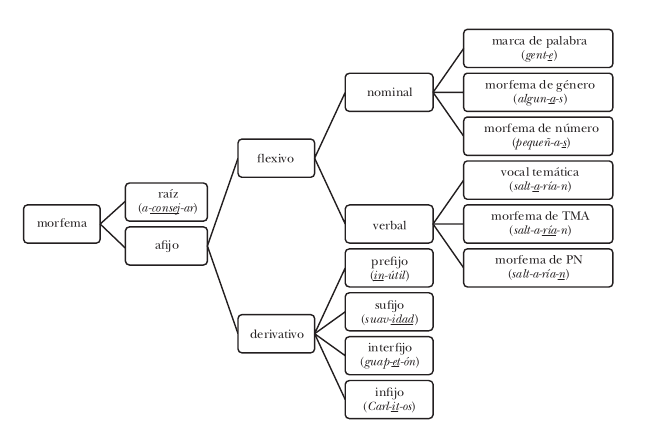
\includegraphics[width=0.75\linewidth]{ESQ02.png}
%     \caption{Tipos de morfemas en el español}
%     \label{fig:tipos_morfemas}
% \end{figure}

Este análisis permite que los sistemas automáticos interpreten y distingan variaciones entre palabras como \textquote{solar} e \textquote{insolación}

\section{Elementos del análisis morfológico}
Para separar una palabra en su lema y morfemas, el análisis morfológico usa 3 elementos principales:

\begin{enumerate}
    \item \textbf{Lexicón:}
    El lexicón es una colección estructurada de palabras y morfemas que incluye información básica sobre su significado y características. Dado que incluir todas las palabras de un idioma es inviable, los lexicones computacionales suelen centrarse en los morfemas. Por ejemplo, pueden indicar si una raíz es un verbo o un sustantivo.
    
    \item \textbf{Hechos morfotácticos:}
    Estos describen las reglas que determinan cómo los morfemas pueden combinarse para formar palabras válidas en un idioma. En español, por ejemplo, los morfemas que indican número plural se colocan después del sustantivo (\textit{niño-s}), mientras que en otros idiomas, podrían aparecer antes.

    \item \textbf{Reglas ortográficas:}
    Las reglas ortográficas modelan los cambios en la forma de los morfemas cuando se combinan. Por ejemplo, al formar el plural de la palabra española \textquote{nuez}, se intercalan cambios en la raíz y se añade \textquote{e} antes del sufijo \textquote{-s}, resultando en \textquote{nueces}. Estas reglas permiten manejar alteraciones específicas en la forma escrita de las palabras.
\end{enumerate}
Estos elementos se combinan para construir sistemas robustos de análisis morfológico capaces de descomponer palabras en sus morfemas y proporcionar su estructura gramatical.

\section{Técnicas de análisis morfológico}
Existen diversas técnicas para abordar el análisis morfológico de manera automática. Entre las más destacadas están:

\begin{enumerate}
    \item {\textbf{Autómatas finitos:}}
    Los autómatas finitos son modelos computacionales que representan el conocimiento morfotáctico en forma de un grafo, donde los estados corresponden a posibles etapas en la formación de palabras, y las transiciones indican combinaciones válidas de morfemas. Por ejemplo, un autómata puede modelar la formación de plurales en español añadiendo el morfema \textquote{-s} al final de un sustantivo. 

    \item{\textbf{Transductores de autómatas finitos:}}
    Los transductores de autómatas finitos extienden los autómatas simples al permitir la traducción entre dos niveles de representación:

    El nivel de superficie, que corresponde a la forma escrita de la palabra (e.g., \textquote{niños}).
    El nivel léxico, que descompone la palabra en sus morfemas (e.g., \textquote{niño +N +Masc +Pl}).
    Este enfoque permite no solo verificar si una palabra es válida, sino también descomponerla en sus componentes gramaticales.

    \item {\textbf{Morfología de dos niveles:}}
    Este modelo incorpora reglas ortográficas directamente en los transductores de estados finitos. Al combinar un lexicón y un conjunto de reglas ortográficas, permite manejar palabras que sufren cambios significativos al unirse morfemas. Por ejemplo, el sistema puede reconocer que \textquote{luz} se convierte en \textquote{luces} en plural, aplicando las reglas de cambio de \textquote{z} a \textquote{c}.

\end{enumerate} 

\section{Ambigüedad}
Un desafío clave en el análisis morfológico es la \textbf{ambigüedad}, que ocurre cuando una palabra tiene múltiples posibles análisis morfológicos. Por ejemplo, la palabra \textquote{vino} puede analizarse de las siguientes maneras:

\begin{itemize}
    \item Como el verbo \textbf{\textquote{venir}}, en tiempo pasado, tercera persona del singular (+V +Perf +3P +Sg).
    \item Como el sustantivo \textbf{\textquote{vino}}, de género masculino y número singular (+N +Masc +Sg).
\end{itemize}
En estos casos, el sistema morfológico no puede decidir cuál análisis es el correcto sin información adicional.

La resolución de esta ambigüedad requiere el uso de \textbf{información externa}, como el contexto en el que aparece la palabra. Por ejemplo, al analizar la frase \textquote{El vino tinto es delicioso}, el artículo \textquote{El} y el adjetivo \textquote{tinto} proporcionan pistas para identificar \textquote{vino} como un sustantivo, no como un verbo.

\chapter{Etiquetado Morfosintáctico (POS Tagging)}
\etocframedstyle[1]{}
\etocsetnexttocdepth{\profundidadIndiceCapitulo}
\localtableofcontents
El etiquetado morfosintáctico, también conocido como POS tagging (del inglés \emph{Part-of-Speech tagging}), es un proceso fundamental en el PLN que consiste en asignar una etiqueta gramatical a cada palabra en un texto.  Estas etiquetas representan la categoría gramatical a la que pertenece cada palabra, como sustantivo, verbo, adjetivo, adverbio, etc.
\section{Categorías Gramaticales}
Las categorías gramaticales, o partes de la oración, son clases de palabras que comparten características morfológicas y sintácticas similares.

\section{Funcionamiento del Etiquetado Morfosintáctico}
El etiquetado morfosintáctico toma como entrada una secuencia de palabras y produce como salida una secuencia de pares formados por la palabra y su correspondiente etiqueta gramatical.
Un ejemplo de esto sería:
\emph{Entrada:} El perro corre rápido.
\emph{Salida:} El/DET perro/N corre/V rápido/ADV
Donde:
\begin{itemize} \item DET: Determinante \item N: Sustantivo \item V: Verbo \item ADV: Adverbio \end{itemize}
Para realizar el etiquetado, se pueden utilizar diferentes conjuntos de etiquetas. Uno de los más utilizados en inglés es el Penn Treebank, que cuenta con 45 etiquetas para identificar las distintas partes de la oración.
\section{Etiquetado Morfosintáctico con Modelos Ocultos de Márkov (HMM)}
Los Modelos Ocultos de Márkov (HMM) son una herramienta estadística que se utiliza para modelar secuencias de datos donde los estados subyacentes no son observables directamente. En el contexto del etiquetado morfosintáctico, los estados ocultos representan las categorías gramaticales y las observaciones son las palabras del texto.
Un HMM para el etiquetado morfosintáctico se compone de:
 \begin{itemize} \item Estados ocultos: Representan las etiquetas gramaticales (categorías). \item Observaciones: Son las palabras del texto. \item Probabilidades de transición: Indican la probabilidad de pasar de una etiqueta a otra. Por ejemplo, la probabilidad de que un determinante (DET) sea seguido por un sustantivo (N). \item Probabilidades de emisión: Representan la probabilidad de que una etiqueta esté asociada a una palabra específica. Por ejemplo, la probabilidad de que la palabra \textquote{el} sea un determinante (DET). \end{itemize}
Para encontrar la secuencia de etiquetas más probable para una secuencia de palabras, se utiliza el algoritmo de Viterbi.  Este algoritmo calcula la ruta más probable a través de los estados ocultos del HMM, considerando las probabilidades de transición y de emisión.
\section{Dificultades del Etiquetado Morfosintáctico}
El etiquetado morfosintáctico automático presenta algunas dificultades, como:
 \begin{itemize} \item Ambigüedad: Una misma palabra puede pertenecer a diferentes categorías gramaticales dependiendo del contexto. \item Necesidad de grandes conjuntos de datos: Los HMM necesitan grandes conjuntos de datos etiquetados para entrenar sus parámetros.
 \end{itemize}
A pesar de estas dificultades, el etiquetado morfosintáctico es una tarea crucial en el PLN, ya que proporciona información fundamental para el análisis sintáctico, semántico y pragmático del lenguaje.

\chapter{Semántica y Representación del Significado}
\etocframedstyle[1]{}
\etocsetnexttocdepth{\profundidadIndiceCapitulo}
\localtableofcontents

Según la RAE, la semántica es la \textquote{Disciplina que estudia el significado de las unidades lingüísticas y de sus combinaciones}\autocite{rae.diccionario}.
Esto conlleva no conocer los atributos de las palabras, sino también su significado completo.
El análisis semántico permite a las máquinas comprender el significado del lenguaje humano, no solo la estructura superficial de las oraciones. 


\section{Niveles de análisis semántico:}

\subsection{Semántica léxica} 
Se centra en el significado de las palabras individuales.

\begin{itemize}
    \item Ejemplo: La palabra "banco" puede tener diferentes significados: una institución financiera, un asiento, etc.
    \item \textbf{Desambiguación del sentido de las palabras (WSD):} Consiste en seleccionar el sentido apropiado de una palabra según el contexto en que aparece.
\end{itemize}

\subsection{Semántica oracional}
Analiza el significado de las oraciones, considerando la composición del significado de las palabras que las componen y sus relaciones sintácticas.

Dos formas:
\begin{itemize}
    \item{Lógica de predicados:} Con lógica formal, se procesa con reglas explícitas.
    \item{Roles semánticos:} Evto + Argumentos. PropBank define roles semánticos como Arg0 (agente), Arg1 (paciente), Arg2 (beneficiario), etc.
\end{itemize}

\begin{itemize}
    \item Principio de composicionalidad: El significado de una expresión compleja está determinado por el significado de sus unidades y las relaciones entre ellas.
    \item PropBank: Es un recurso lingüístico que describe las relaciones semánticas entre los verbos y sus argumentos.
\end{itemize}

Ejemplo: En la oración \textquote{La policía militar arrestó a tres personas}, \textquote{La policía militar} sería Arg0 (agente) y \textquote{a tres personas} sería Arg1 (paciente).

\subsection{Semántica textual}
Estudia el significado de unidades lingüísticas más grandes, como párrafos y textos completos. Este nivel considera la cohesión y la coherencia del discurso.

\section{Formas de representar el significado}
\begin{itemize}
    \item {Lógica de primer orden:}
        Utiliza fórmulas lógicas con cuantificadores, predicados y variables para representar el significado.
    \item{Redes semánticas:}
        Representa el conocimiento como un grafo, donde los nodos representan conceptos y las aristas relaciones entre ellos.
    \item {Diagramas de dependencias conceptuales: }
        Proporcionan una representación gráfica de las dependencias conceptuales\autocite{SCHANK1972552}.
    \item {Basados en frames:}
        Representa el conocimiento en estructuras de datos que contienen información sobre conceptos y sus atributos.
        Funcionan rellenando \textquote{\textit{huecos}} (slots) en \textquote{\textit{plantillas}} (frames)\autocite{Fillmore1985FramesAT}.
\end{itemize}
\subsection{Lógica descriptiva}
Combina la lógica de primer orden con la representación intuitiva de las redes semánticas. Es la base formal de la web semántica. Podría considerarse como un subconjunto de la lógica de primer orden.







\chapter{Pragmática}
\etocframedstyle[1]{}
\etocsetnexttocdepth{\profundidadIndiceCapitulo}
\localtableofcontents


La pragmática estudia la influencia del contexto en la interpretación del significado. Se centra en cómo el lenguaje se utiliza en situaciones específicas para lograr objetivos comunicativos.
Por esto, el contexto es fundamental para comprender el significado completo de un enunciado, ya que proporciona información adicional sobre las intenciones del hablante y la situación comunicativa.

Esta información va contenida en los actos de habla, que pueden clasificar en tres categorías:
\begin{enumerate}
    \item {Locutivo:} Acto mismo de emisión de sonidos que pueden ser interpretados de manera literal por el interlocutor.
    \item{Ilocutivo:} Intención o finalidad subyacente a la oración.
    \item{Perlocutivo:} Efectos producidos al interlocutor por actos ilocutivos.
\end{enumerate}

\section{Principio de cooperación de Grice}
Establece que los hablantes cooperan en una conversación para lograr una comunicación efectiva.
Las máximas son las que siguen:
\begin{enumerate}
    \item {Cantidad:} Proporcionar la cantidad (1) de información adecuada (2).
    \item {Calidad:} Decir la verdad (1) y tener pruebas para las afirmaciones (2).
    \item {Relación:} Ser relevante al tema de la conversación.
    \item {Modo:}  Ser claro (1), breve (2), ordenado (3) y evitar la ambigüedad (4).
\end{enumerate}

Como muchas veces se usan significados implicitos, se crea la palabra:
\paragraph{Implicaturas:}Son los significados implícitos que se infieren a partir de lo que se dice explícitamente y del contexto.
Tienen dos tipos: \textbf{Convencionales} y \textbf{no convencionales}.

El uso de las implicaturas flexibiliza las \textbf{máximas} y alza el mínimo para la consideración de violación de las máximas.

\section{Formas de cortesía}
La cortesía es una forma de comunicarse que se ayuda de estrategias para evitar malentendidos u ofender a la contraparte en una conversación.
Se definen como normas de cortesía: \textbf{no imponer}, \textbf{dar opciones} y \textbf{hacer sentir bien al interlocutor}.
En ocasiones, la cortesía puede llevar a romper las máximas de Grice para evitar ofender al interlocutor.

\section{Análisis conversacional}
Estudia las características y tipos de conversaciones.

Formatos de las conversaciones:
\begin{itemize}
    \item Interactiva: Implica la participación de dos o más personas.
    \item Dinámica: Implica un intercambio continuo de roles entre hablante y oyente.
    \item Cooperativa: Los interlocutores trabajan juntos para lograr una comunicación efectiva.
\end{itemize}

Tipos de conversaciones:
\begin{itemize}
    \item Coloquial: Se caracteriza por el uso de un lenguaje informal.
    \item Formal: Se caracteriza por el uso de un lenguaje más cuidado y preciso.
    \item Simétrica: Los participantes tienen el mismo estatus comunicativo.
    \item Asimétrica: Los participantes tienen diferente estatus comunicativo, como en una entrevista o una consulta médica.
    \item Privada: Ocurre en un ámbito personal entre hablantes que se conocen bien.
    \item Pública: Ocurre entre personas que no se conocen bien y el contenido no es íntimo.
    \item Abierta: Hay otras personas presentes como oyentes que pueden participar en la conversación.
    \item Cerrada: Se limita a dos participantes.
    \item Vía chat: Presenta características particulares, como la oralización del texto y la escritura sincrónica.
\end{itemize}

\subsection{Importancia de la pragmática en los chatbots}
Para que los chatbots puedan mantener conversaciones naturales, deben ser capaces de:

\begin{itemize}
    \item Comprender el contexto.
    \item Inferir información implícita.
    \item Identificar las intenciones del usuario.
    \item Adaptar su lenguaje a la situación comunicativa.
\end{itemize}


\chapter{Semántica vectorial}
\etocframedstyle[1]{}
\etocsetnexttocdepth{\profundidadIndiceCapitulo}
\localtableofcontents

Nueva aproximación formal, representa \textbf{palabras y documentos} como \textbf{vectores} en un espacio multidimensional, donde la \textbf{distancia entre vectores} refleja la \textbf{similitud semántica}. 

\paragraph{Dimensiones lingüísticas:} El espacio vectorial tiene múltiples dimensiones, donde cada dimensión representa un contexto lingüístico. 

\paragraph{Factores que influyen en la representación vectorial:}
\begin{enumerate}
    \item Representación del contexto: Define las dimensiones del espacio vectorial.
    \item Representación de las palabras: Cómo se codifican las palabras como vectores.
    \item Cálculo de pesos: Asigna pesos a las palabras según su importancia en el contexto.
\end{enumerate}
\section{Representación del contexto}
Se puede acotar el contexto mediante:
\begin{enumerate}
    \item Matriz término-documento: Representa la frecuencia de las palabras en un conjunto de documentos.
            Limitaciones:  No captura las relaciones semánticas entre palabras que no aparecen en el mismo documento.
    \item Matriz de co-ocurrencias: Representa la frecuencia con la que dos palabras aparecen juntas en un contexto definido (por ejemplo, una ventana de palabras).
        Ventajas:  Captura relaciones semánticas entre palabras que no necesariamente aparecen en el mismo documento

\end{enumerate}

\section {Representación de las palabras}

Se pueden utilizar diferentes métodos para codificar las palabras como vectores:

\begin{itemize}
    \item One-hot encoding: Cada palabra se representa como un vector binario con un único 1 en la posición correspondiente a la palabra.
    \item Tokens: Se asignan identificadores numéricos a las palabras.
    \item Raíz (stem): Se reduce la palabra a su raíz.
    \item Lemas: Se utiliza la forma canónica de la palabra.
    \item Información gramatical: Se incluye la categoría gramatical o la función sintáctica.
\end{itemize}

\section {Cálculo de pesos}
\begin{itemize}
    \item Frecuencias absolutas: Número de veces que la palabra aparece en el contexto.
    \begin{itemize}
        \item Limitaciones: No considera la importancia relativa de la palabra en el contexto.
    \end{itemize}
    \item Frecuencias relativas: Proporción de veces que la palabra aparece en el contexto.
    \begin{itemize}
        \item Limitaciones: No considera la importancia relativa de la palabra en el contexto.
    \end{itemize}
    \item TF/IDF (\textit{Term Frequency-Inverse Document Frequency}): Combina la frecuencia del término en el documento con la frecuencia inversa del término en el corpus.
    \begin{itemize}
        \item Ventajas: Da más peso a las palabras que son específicas de un documento.
    \end{itemize}
    \item PMI (\textit{Pointwise Mutual Information}): Mide la asociación entre dos palabras.
\end{itemize}

\section{Word Embeddings}
 Representaciones vectoriales densas de palabras que capturan relaciones semánticas y sintácticas.
 
Ventajas:
\begin{itemize}
    \item Representaciones compactas: Reducen la dimensionalidad del espacio vectorial, lo que facilita el procesamiento.
    \item Captura de relaciones semánticas: Palabras con significado similar tienen vectores cercanos en el espacio vectorial.
\end{itemize}

\paragraph{Word2Vec:} Un modelo popular para generar Word Embeddings.
\begin{itemize}
    \item Funcionamiento: Entrena un clasificador para predecir la probabilidad de que una palabra aparezca cerca de otra.
    \item Auto-supervisión: Utiliza un corpus de texto sin necesidad de anotaciones manuales.
    \item Interpretación: La distancia entre los vectores de dos palabras refleja su similitud semántica.
\end{itemize}


\chapter {Agentes conversacionales y chatbots}
\etocframedstyle[1]{}
\etocsetnexttocdepth{\profundidadIndiceCapitulo}
\localtableofcontents

\textquote{Los agentes conversacionales, también llamados sistemas de diálogo, son programas que conversan con las personas a través del lenguaje natural.}

\section{Tipos de agentes conversacionales}
Existen dos tipos principales de agentes conversacionales:

\subsection{Agentes conversacionales dedicados}
Se centran en la ejecución de una tarea específica dentro de un dominio determinado.

Mantienen conversaciones cortas y sencillas, generalmente de una a unas pocas interacciones.  Ejemplos de estos agentes son los asistentes virtuales como Siri, Google Assistant o Alexa, que ayudan con tareas como programar alarmas, enviar mensajes o controlar electrodomésticos.
También son utilizados por empresas para atender a sus clientes en sitios web.

\subsection{Chatbots}
Permiten mantener conversaciones más extensas y no estructuradas sobre cualquier tema.
Su objetivo es ofrecer una experiencia conversacional realista con el usuario.

Un ejemplo es Mitsuku, ganador del Premio Loebner por su capacidad de simular una conversación humana. 
Es importante diferenciar los chatbots de los agentes conversacionales dedicados, ya que los chatbots se enfocan en la naturalidad de la conversación más que en la ejecución de una tarea específica.

\section{Características de las conversaciones entre humanos}
Para que los agentes conversacionales puedan simular una conversación humana de manera convincente, es necesario que imiten las características clave de las conversaciones entre personas:

\begin{itemize}
    \item \textbf{Turnos de palabra:} Las conversaciones se componen de turnos de palabra consecutivos que alternan las opiniones de los participantes. Para los agentes conversacionales, manejar los turnos de palabra y los tiempos de respuesta es una tarea compleja. El análisis conversacional estudia la gestión de turnos mediante reglas que modelan el intercambio en los momentos de transición (TRP: Transition Relevance Places).
    \item \textbf{Actos de habla:} Cada expresión en una conversación puede interpretarse como una acción que realiza el interlocutor. La teoría de los actos de habla, desarrollada por John L. Austin, clasifica estas acciones en diferentes tipos. Para los agentes conversacionales, la interpretación de los actos de habla y la generación de respuestas adecuadas no es una tarea trivial.
    \item \textbf{Puntos de coincidencia:} Para que una conversación se desarrolle con éxito, los interlocutores deben establecer puntos de coincidencia, es decir, asegurarse de que ambos comprenden el significado y la intención de las expresiones del otro. En las conversaciones entre humanos, esto se logra mediante asentimientos, reformulaciones, preguntas de confirmación y otras señales de comprensión. Los agentes conversacionales deben imitar estos comportamientos para asegurar la fluidez de la conversación y evitar confusiones.
    
    \item \textbf{Estructura de la conversación:} Si bien las conversaciones tienen una estructura libre, se pueden identificar patrones como los pares adyacentes (pregunta-respuesta, propuesta-aceptación, etc.). Estos patrones ayudan a los agentes conversacionales a predecir el tipo de respuesta que se espera en cada turno y facilitan la generación automática de diálogos. Además de los pares adyacentes, existen otros patrones que definen la estructura de conversaciones específicas, como las llamadas telefónicas.
    
    \item \textbf{Información implícita:}  el significado de una contribución no se limita al significado de las palabras entendidas de forma individual; el receptor del mensaje puede inferir información.
\end{itemize}

\section{Arquitectura}
Los agentes conversacionales, siguen una estructura básica común:
\begin{itemize}
    \item Reconocimiento automático del habla (opcional): módulo de entrada que extrae las palabras a partir de la señal de audio grabada
    \item Comprensión del lenguaje natural: módulo que realiza tareas de procesamiento del lenguaje natural para extraer la semántica de las frases que recibe
    \item Gestión del diálogo: módulo principal del agente que identifica la acción que debe realizar el agente en el siguiente turno de palabra y cómo se debe continuar la conversación
    \item Generación del lenguaje natural: módulo que elige los conceptos que se quieren expresar al usuario y, además, planifica cómo expresarlos en palabras
    \item Conversión del texto al habla: módulo de salida que sintetiza en formato de voz el mensaje a transmitir al usuario en el siguiente turno de palabra
\end{itemize}

\section{Diseño}
Los chatbots, agentes conversacionales que permiten reproducir conversaciones extensas y no estructuradas, se dividen en dos clases según su implementación: basados en reglas y basados en corpus.

\subsection{Chatbots Basados en Reglas}
Los chatbots basados en reglas utilizan reglas patrón \(\rightarrow\) transformación. Cada regla describe la transformación que se debe aplicar a la declaración hecha por el usuario para obtener la respuesta que le va a proporcionar el chatbot. Un chatbot basado en reglas es ELIZA, diseñado para simular a un psiquiatra que hace reflexionar al paciente devolviéndole sus propias declaraciones.

\subsection{Chatbots Basados en Corpus}
Los chatbots basados en corpus aplican técnicas de minería de datos a grandes conjuntos de conversaciones entre humanos. Se dividen en dos tipos:
\begin{itemize}
    \item basados en recuperación de información: obtienen una respuesta proporcionada por un humano en una conversación previa.
    \item chatbots secuencia a secuencia: basados en el paradigma de la traducción automática, utilizan técnicas de aprendizaje automático supervisado.
\end{itemize}

\section{Frames en Agentes Conversacionales}
Los frames son una estrategia de representación. Los agentes conversacionales basados en frames utilizan una ontología para la representación formal de la semántica. Esta ontología define los frames (plantillas para una frase), los slots (huecos en cada plantilla) y los posibles valores para rellenar estos huecos. La información dentro de los frames se organiza en pares atributo-valor, que restringen la tipología semántica de los valores que pueden ir asociados a cada hueco en la plantilla. El módulo de comprensión del lenguaje natural de un agente conversacional basado en frames extrae la semántica de la petición lanzada por el usuario identificando diferentes elementos:
\begin{itemize}
    \item Dominio: a qué se refiere el usuario (reservar vuelos, programar la alarma)
    \item Intención: qué quiere hacer el usuario (consultar precios, reservar un vuelo)
    \item Valores de los slots: información específica de la petición (origen, destino, fecha)
\end{itemize}
El módulo de comprensión del lenguaje natural también debe identificar otros aspectos propios del diálogo como los puntos de coincidencia (turnos de confirmación, negación, cortesía, etc.).

Para extraer la semántica de la petición, se utilizan técnicas de procesamiento del lenguaje natural como:
\begin{itemize}
    \item Gramáticas de unificación: utilizan una ontología para la representación formal de la semántica de la conversación.
    \item Gramáticas semánticas: gramáticas libres de contexto en las que la parte izquierda de las reglas aparecen los conceptos semánticos.
    \item Aprendizaje automático supervisado: entrena un clasificador para asignar a cada oración su dominio e intenciones, y generar un modelo que mapee la frase a los valores de los slots.
    \item Modelo HMM semántico: modelo probabilístico donde los estados ocultos son las etiquetas de los slots, y las palabras son los valores que rellenan los slots.
\end{itemize}
 

\printbibliography

\end{document}
